\section{Processing manager}

Processing manager is the major component in the processing of a HLASM source file. It decides which stream of statements is about to be processed and assigns it to the correct processor. It contains components responsible for instruction interpretation as well as instruction format validation. 

\begin{figure}
	\centering
	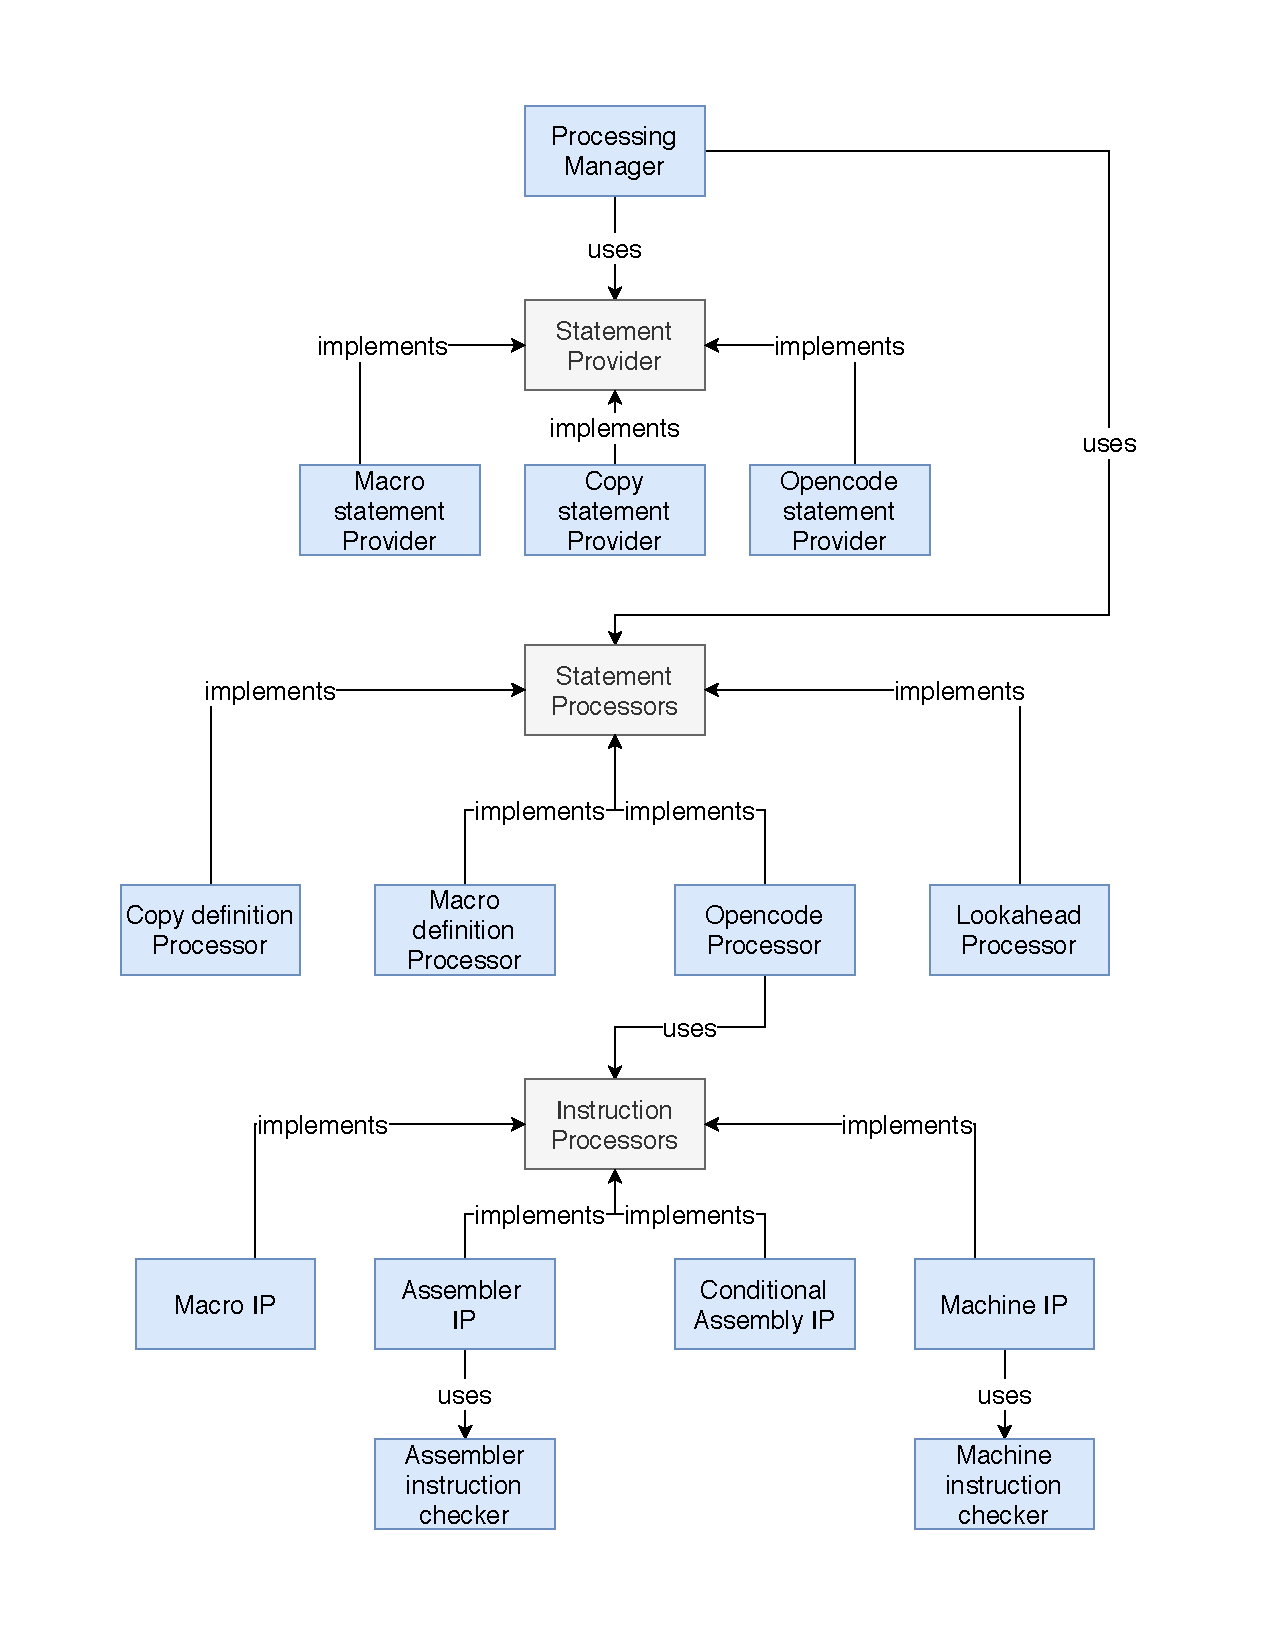
\includegraphics[width=\textwidth]{img/processing_manager_arch}
	\caption{The architecture of Processing manager}
	\label{fig06:proc_mngr}
\end{figure}

\subsection{Overview}

To construct processing manager, analyzer passes this objects to the constructor:
\begin{itemize}
	\item \emph{Parser} that provide statements from the processed file. Further on we will refer to the parser as to the \emph{Opencode statement provider}.
	\item \emph{HLASM context tables} that holds current state of the parsed source.
	\item \emph{Name} of the processed file.
	\item \emph{Parse library provider} to solve in file dependencies.
	\item \emph{Statement fields parser} for parsing deferred statements (see ??). 
\end{itemize}

As the processing of the HLASM source file is rather complicated, we defined a \emph{statement provider} for each different source of statements (see ?? \todo{add section for source of statements in chapter 2}) and a \emph{statement processor} for each different manner of statement processing (see ?? \todo{add section for different processings in chapter 2}). 

Processing manager captures this behaviour. Hence, it contains two arrays, each consisting of different implementation of statement processor, or statement provider (see \cref{fig06:proc_mngr}).  Also, it has notion of the processor or provider that is in the current use and implement interfaces that change them.

\subsection{The main loop}

The main loop of the processing works with the current processor and provider. As the names suggest, statement provider provides next statement for statement processor that processes it accordingly. The loop breaks when the last processor finishes work.

However, the think the reader should focus on is when the current provider/processor is changed. The rules are:

\begin{enumerate}
	\item When the processor finished its work, the next processor is selected from the array.
	\item When the provider finished, before the next provider is selected from the array, manager checks whether the provider's end triggers finishing of the current processor as well. If true, performs rule 1.
\end{enumerate}

\subsection{Statement Providers}

In the processing manager, statement providers are stored in the array based on the priority (lower index, greater priority).

\begin{enumerate}
	\item Macro definition statement provider
	\item Copy definition statement provider
	\item Opencode statement provider
\end{enumerate}

Every cycle of the processor's main loop, each provider is checked --- whether it has statements to provide --- based on the priority. It is because after each cycle, a processor with greater pirority than the current one can be activated.





\subsection{Expressions}
overview

they are parsed in grammar, later you give an expression "symbol evaluator" and it returns its value



\subsection{Data definition}

validation and processing purpose